Insieme alla entità del gioco, ho iniziato a realizzare un semplice sistema di coordinate per gestire movimenti nell'arena, tenendo conto delle premesse fatte in fase di design:
\begin{itemize}
    \item la mappa di gioco deve essere rappresentata logicamente da una griglia;
    \item la mappa di gioco deve avere un contorno non attraversabile (Wall) e un'area di gioco interna (Floor);
    \item ogni entità all'interno dell'arena è caratterizzata da una posizione;
    \item ogni posizione si compone di un punto 2D e di una direzione (opzionale);
    \item ogni entità può muoversi solo in quattro direzioni;
    \item le coordinate possono essere solo numeri interi positivi.
\end{itemize}

Successivamente ho implementato la classe Arena, contenente le entità che popolano la mappa in un dato momento della partita: infatti, il contenuto delle strutture dati di Arena rappresenta una fotografia dello stato del gioco. Si noti la differenza tra Player, che rappresenta l'utente, e Hero, che invece rappresenta il personaggio giocabile. Alcuni componenti dell'arena, vista la loro natura statica, vengono inizializzati con le loro posizioni in fase di creazione, mentre il resto viene gestito da una funzione generateMap() che viene richiamata nella fase di popolazione iniziale, ovvero all'inizio di ogni livello, e da una funzione updateMap() che invece si occupa dell'aggiornamento dello stato di ogni entità e che viene richiamata dal controller ad ogni step logico.

La classe ha come parametri il nome del profilo associato alla partita corrente ed un MapGenerator, ovvero una classe che incapsula la logica di generazione. MapGenerator viene inizializzata con la difficoltà della partita e serve ad implementare il legame tra la difficoltà del gioco (rappresentata da un insieme di valori e range) ed il modo randomico con cui vengono generate le entità.
\begin{figure}[H]
  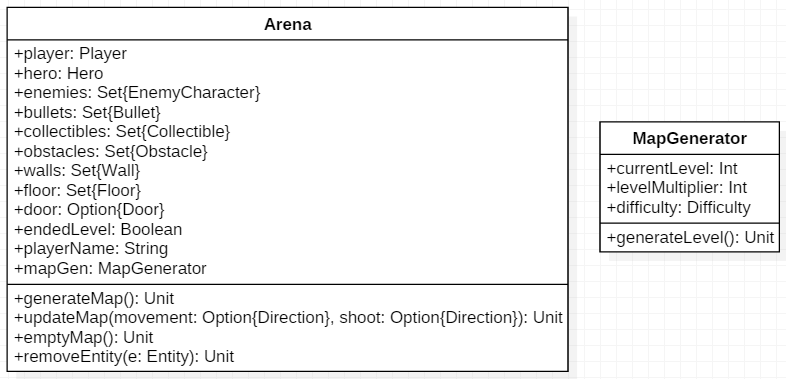
\includegraphics[width=15cm]{res/arenaClass.png}
  \caption{La classe Arena}
  \label{arenaCLass}
\end{figure}

Vista l'importanza logica di Arena, è anche necessario fornire metodi per permettere a classi esterne di lavorare con l'area di gioco. Per lo scopo, il companion object della classe contiene tutti i metodi che possono essere utili alle entità esterne per controllare lo stato del gioco, nonchè per il testing. Una parte fondamentale dello sviluppo è stata la scelta del tipo di funzioni da implementare in questo caso, che ha portato a refactoring in parti diverse dell'implementazione, dovuto soprattutto alla separazione tra funzioni della classe e del companion object e a scelte legate alle strutture dati utilizzate.
\begin{figure}[H]
  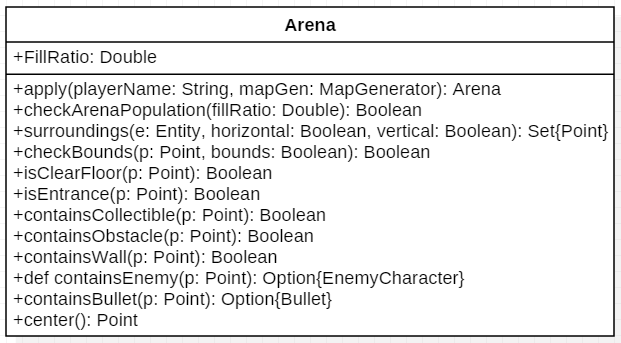
\includegraphics[width=15cm]{res/arenaObject.png}
  \caption{Il companion object della classe Arena}
  \label{arenaObject}
\end{figure}